% last updated in April 2002 by Antje Endemann
% Based on CVPR 07 and LNCS, with modifications by DAF, AZ and elle, 2008 and AA, 2010, and CC, 2011; TT, 2014; AAS, 2016

\documentclass[runningheads]{llncs}
\usepackage{graphicx}
\usepackage{amsmath,amssymb} % define this before the line numbering.
\usepackage{ruler}
\usepackage{color}
\usepackage[caption=false]{subfig}
\usepackage[width=122mm,left=12mm,paperwidth=146mm,height=193mm,top=12mm,paperheight=217mm]{geometry}
\begin{document}
% \renewcommand\thelinenumber{\color[rgb]{0.2,0.5,0.8}\normalfont\sffamily\scriptsize\arabic{linenumber}\color[rgb]{0,0,0}}
% \renewcommand\makeLineNumber {\hss\thelinenumber\ \hspace{6mm} \rlap{\hskip\textwidth\ \hspace{6.5mm}\thelinenumber}}
% \linenumbers
\pagestyle{headings}
\mainmatter
\def\ECCV18SubNumber{27}  % Insert your submission number here

\title{Directional Pseudo-color Enhancement of Image Gradients} % Replace with your title

\titlerunning{ECCV-18 submission ID \ECCV18SubNumber}

\authorrunning{ECCV-18 submission ID \ECCV18SubNumber}

\author{Anonymous ECCV submission}
\institute{Paper ID \ECCV18SubNumber}


\maketitle

\begin{abstract}
Computing an image gradient is a common image filtering task in computer vision and is used to quantify the magnitude and direction of the edges in an image. Typically, the image gradient is represented as a grayscale image. This paper presents an approach to color the edges of an image (the image gradient) in a deliberate, coherent, and artistic manner. By using the direction of the image gradient to pseudo-color the magnitude of the image gradient, we can enhance the visual quality of the gradient. The result is an image that resembles a skeleton of the original image, colored consistently according to edge direction and contrasted against a black background.
\keywords{image filtering, edge detection, pseudo-coloring}
\end{abstract}

\section{Introduction}

Edge detection is a fundamental image processing technique that uses an image gradient to quantify the magnitude and direction of the edges in an image. In this paper, we introduce a technique to color the edges of an image in a deliberate, coherent, and artistic manner. An example is shown in Figure 1.

\begin{figure}
\centering
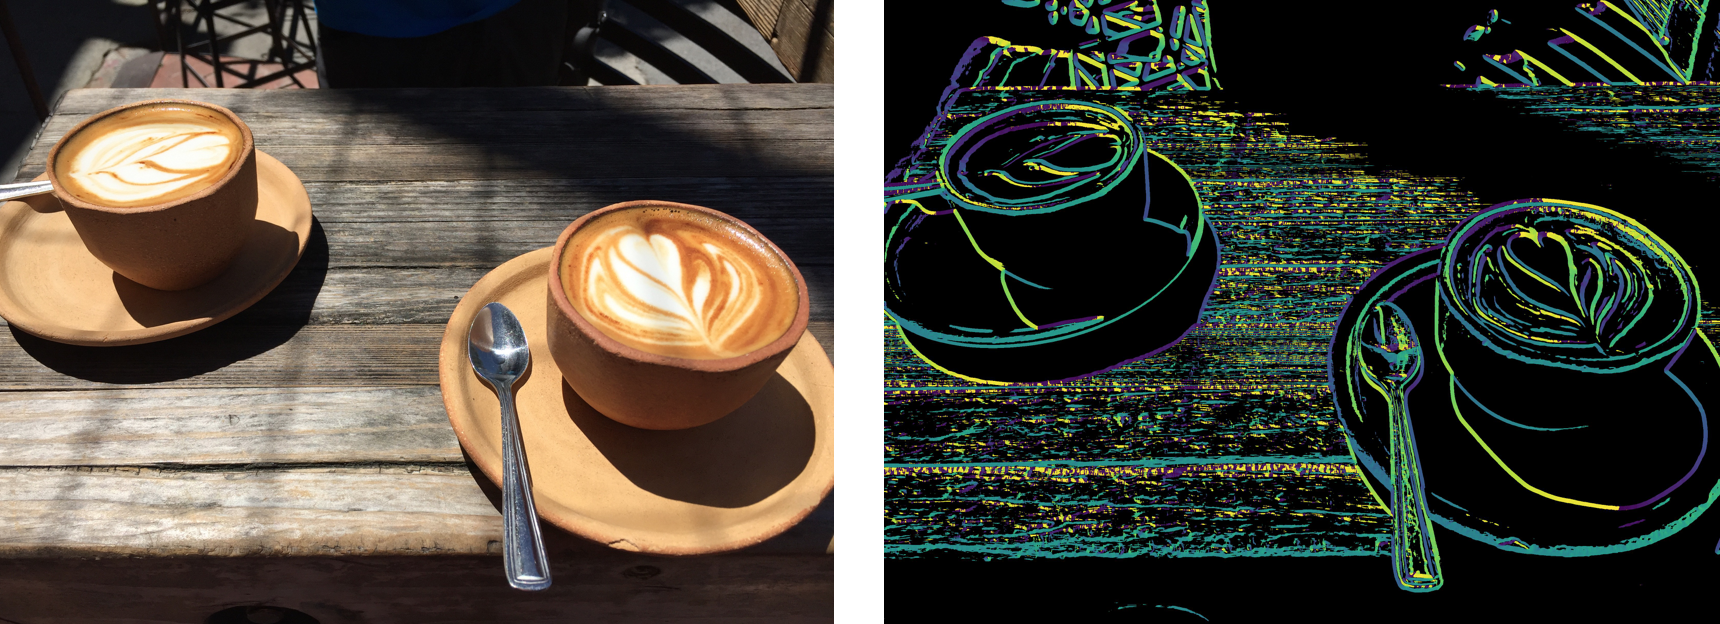
\includegraphics[height=4.4cm]{images/intro.png}
\caption{A demonstration of the approach. Left: The original image. Right: The image gradient magnitude pseudo-colored by the image gradient direction.}
\label{fig:example}
\end{figure}

Image gradients are important because they serve as components for various downstream tasks in computer vision such as edge detection and image classification. However, the image gradients themselves are dull. Image gradients are typically represented as grayscale or black-and-white images depicting the change in intensity at each pixel of the original image, as in the right-hand panel of Figure 2.

\begin{figure}
\centering
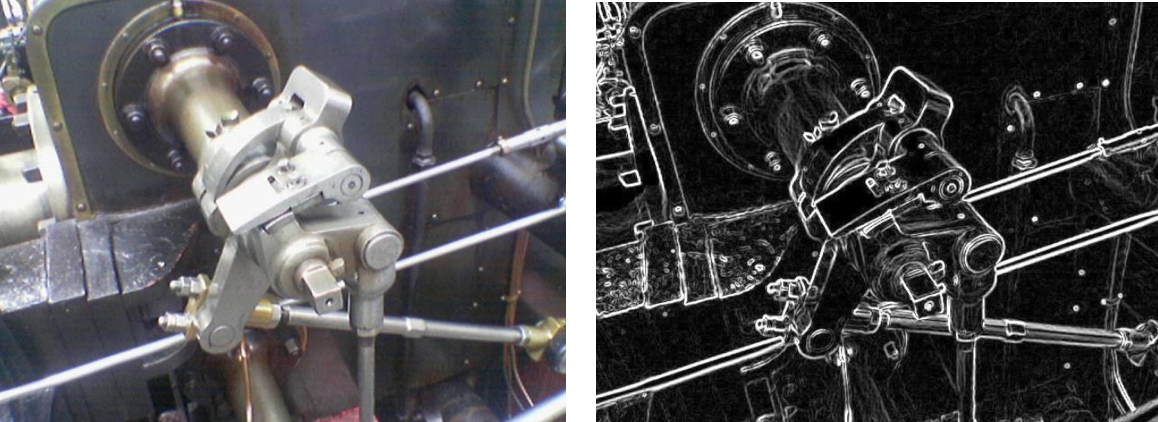
\includegraphics[height=4cm]{images/image_gradient.png}
\caption{The image gradient magnitude (right) is a grayscale image showing the change in intensity at each pixel of the original image (left).}
\label{fig:example}
\end{figure}

The goal of this paper is to make image gradients more appealing and informative by enhancing them with color. The human eye can discern only two-dozen shades of gray, but thousands of shades of color \cite{human_machine}. So, a better, more visible image gradient will reveal details that were not visible in the grayscale gradient. Further, we hope that a colored image gradient will create an artistic rendering of the original image that is aesthetically pleasing.

\section{Methodology}

The proposed pipeline for coloring the edges of an image has two main parts: edge detection and edge coloring.

\subsection{Edge detection}

The standard approach for edge detection is to convolve an image with a derivative filter like the Sobel filter to differentiate the intensity of the image pixels with respect to the horizontal and vertical directions of the image. However, since differentiation is very sensitive to noise, it is useful to blur the image first \cite{filtering_lecture}. This can be achieved by convolving the original image $f$ with a blur filter, such as the Gaussian filter, to produce a blurred image $f_b$. For the purposes of edge detection, we will first convert $f$ to a grayscale image. Figure 3 shows the blur transformation.

\begin{align}
f_b = f * \begin{bmatrix} 
1 & \quad 2 & \quad 1 \\ 
2 & \quad 4 & \quad 2 \\ 
1 & \quad 2 & \quad 1  
\end{bmatrix}
\end{align}

\begin{figure}
\centering
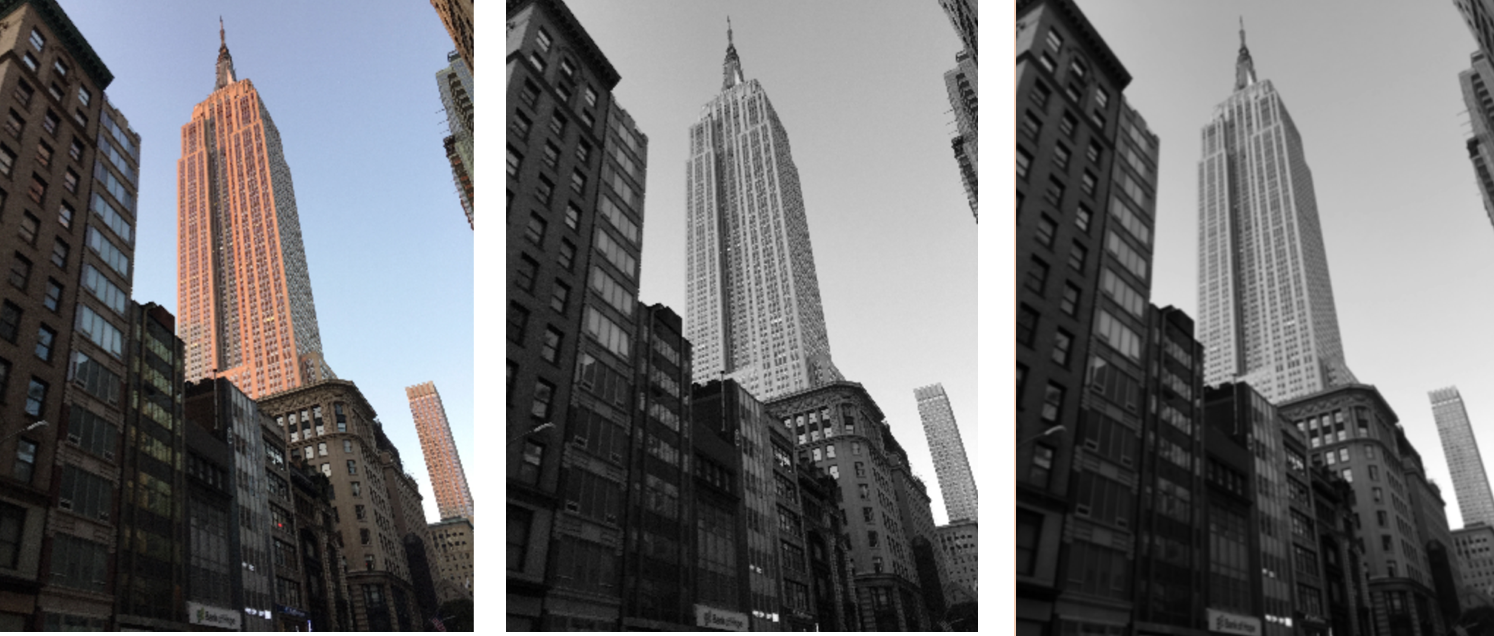
\includegraphics[height=5cm]{images/blur.png}
\caption{Blurring denoises the image and makes it easier to detect edges. The original image (left) is converted to grayscale (middle) and then blurred (right) using a blur filter.}
\label{fig:example}
\end{figure}

Once the image has been blurred, we can perform edge detection using Sobel filters \cite{sobel}. We convolve the blurred image $f_b$ with the horizontal and vertical Sobel filters, $S_x$ and $S_y$ respectively, to approximate the image derivatives in the horizontal and vertical directions, $\frac{\partial f_b}{\partial x}$ and $\frac{\partial f_b}{\partial y}$ respectively. $\frac{\partial f_b}{\partial x}$ has a strong response to vertical edges, and $\frac{\partial f_b}{\partial y}$ has a strong response to horizontal edges.

\begin{align}
S_x = \begin{bmatrix} 
1 & \quad 0 & \quad -1 \\ 
2 & \quad 0 & \quad -2 \\ 
1 & \quad 0 & \quad -1  
\end{bmatrix}
\quad S_y = \begin{bmatrix} 
1 & \quad 2 & \quad 1 \\ 
0 & \quad 0 & \quad 0 \\ 
-1 & \quad -2 & \quad -1  
\end{bmatrix}
\end{align}

\begin{align}
\frac{\partial f_b}{\partial x} &= f_b * S_x \\
\frac{\partial f_b}{\partial y} &= f_b * S_y
\end{align}

$\frac{\partial f_b}{\partial x}$ and $\frac{\partial f_b}{\partial y}$ can be combined to form the image gradient $\nabla f_b$. The following equations show how to calculate the magnitude $G$ and the direction $\theta$ of the image gradient. The resulting image gradient magnitude represents the intensity of edges in the image and is displayed in Figure 4. 

\begin{align}
\nabla f_b &= \begin{bmatrix} \frac{\partial f_b}{\partial x}, \frac{\partial f_b}{\partial y} \end{bmatrix} \\
G &= \vert \vert \nabla f_b \vert \vert = \sqrt{\Big( \frac{\partial f_b}{\partial x} \Big)^2 + \Big( \frac{\partial f_b}{\partial y} \Big)^2} \\
\theta &= tan^{-1} \Big(\frac{\partial f_b}{\partial x} / \frac{\partial f_b}{\partial y})
\end{align}

\begin{figure}
\centering
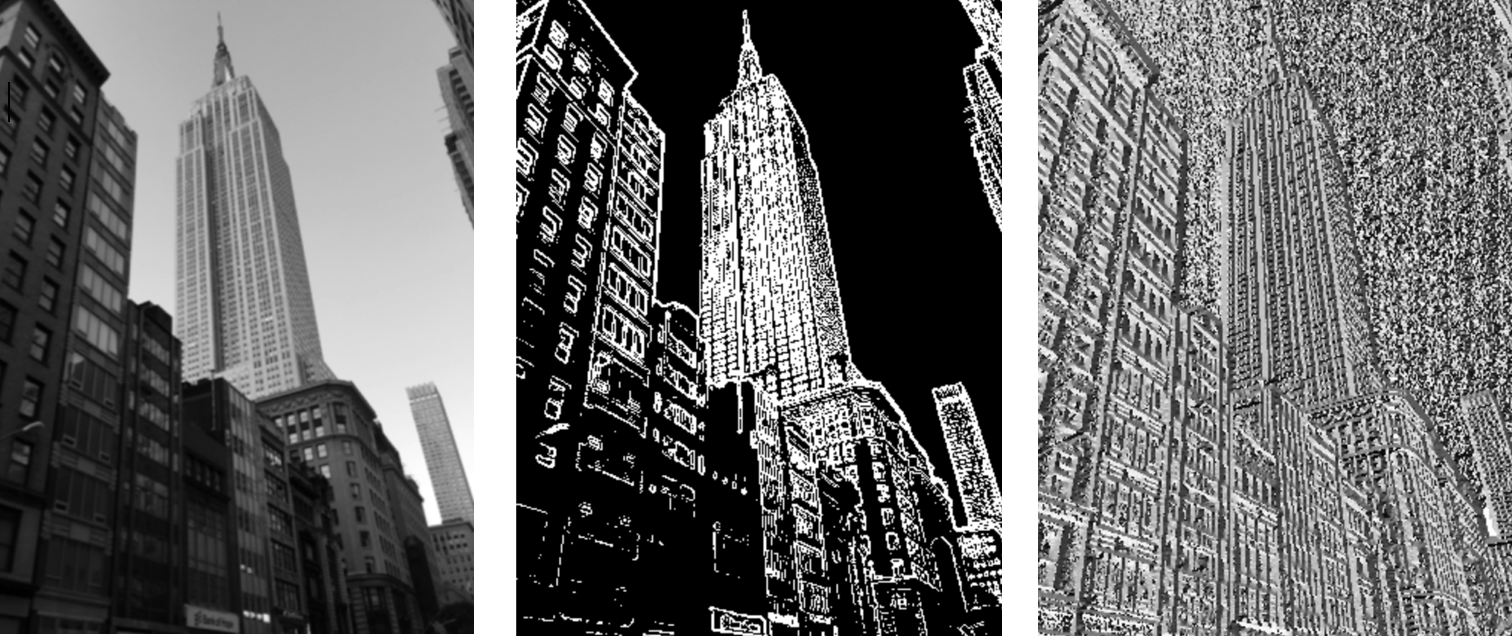
\includegraphics[height=5cm]{images/edge.png}
\caption{Edge detection using Sobel filters. We convolve the blurred image (left) with the Sobel filters and compute the magnitude (middle) and direction (right) of the gradient.}
\label{fig:example}
\end{figure}

\subsection{Edge coloring}

Once the edges have been detected, there are potentially many ways to color them. One approach is to color the edges using the same colors from the original image, esentially masking the (thresholded) gradient magnitude image over the original image. However, this would not add any novelty to the resulting image.

Instead, we choose to pseudo-color the gradient magnitude image using values from the gradient direction image. Pseudo-coloring is the process of mapping the shades of gray in a grayscale image to colors using a color map \cite{pseudo_color}. A color map, defined in line (8), is a function that maps normalized numerical values to RGB pixel values along some color spectrum \cite{color_map}. Figure 5 shows examples of color maps available in the Python Matplotlib library.

\begin{align}
color\_map: [0, 1] \rightarrow (R \in [0,1], G \in [0,1], B \in [0,1])
\end{align}

\begin{figure}
\centering
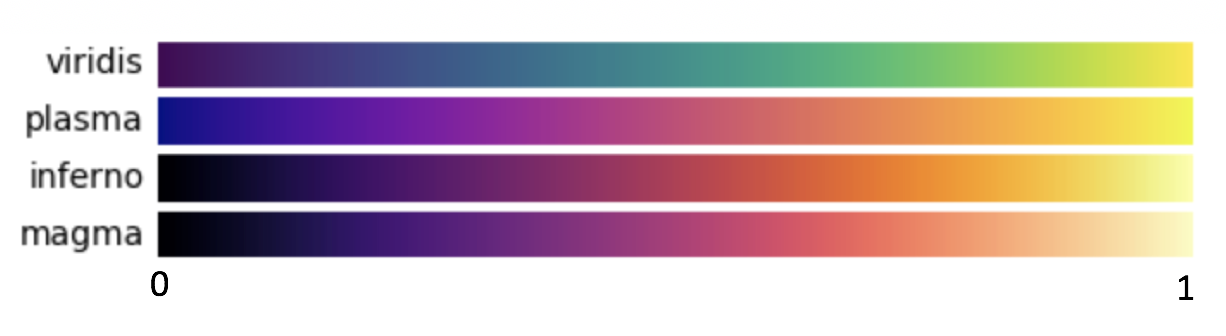
\includegraphics[height=2cm]{images/color_map.png}
\caption{Color maps in the Python Matplolib library.}
\label{fig:example}
\end{figure}

After selecting a color map, we transform our gradient magnitude and direction to prepare them for coloring. First, in line (9), we threshold the gradient magnitude image, converting pixel $G_{x,y}$ to 1 if it has intensity above a threshold value $t$, and 0 otherwise. This thresholding turns the gradient magnitude into a black-and-white image $T$. Then, in line (10), we mask the thresholded gradient magnitude over the gradient direction to create the colored image C. If $T_{x,y}$ is 0, then the pixel $C_{x, y}$ becomes a black pixel (R=0, B=0, G=0). Otherwise, if $T_{x,y}$ is 1, we normalize the pixel's gradient direction $\theta_{x, y}$ between 0 and 1 and apply the color map to color pixel $C_{x, y}$. As a result, C is an image of the thresholded gradient magnitude pseudo-colored by the normalized gradient direction.

\begin{align}
T_{x,y} = \left\{
  \begin{array}{lr}
    1 \quad \text{if  } G_{x,y} \geq t \\
    0 \quad \text{otherwise}
  \end{array}
\right.
, \forall x \in X, \forall y \in Y
\end{align}

\begin{align}
C_{x,y} = \left\{
  \begin{array}{lr}
    color\_map \Big(\frac{\theta_{x,y} - min(\theta)}{max(\theta)} \Big) \quad \text{if  } T_{x,y} = 1 \\
    (R=0, B=0, G=0) \quad \text{otherwise}
  \end{array}
\right.
, \forall x \in X, \forall y \in Y
\end{align}

Because of this directional pseudo-coloring, edges along the same direction are assigned the same color, adding consistency and coherency to the image. The resulting image is also surprisingly novel, with edges of multiple colors against a black background that makes it very different from the original image. An example of the coloring is shown in Figure 6.

\begin{figure}[h!]
\centering
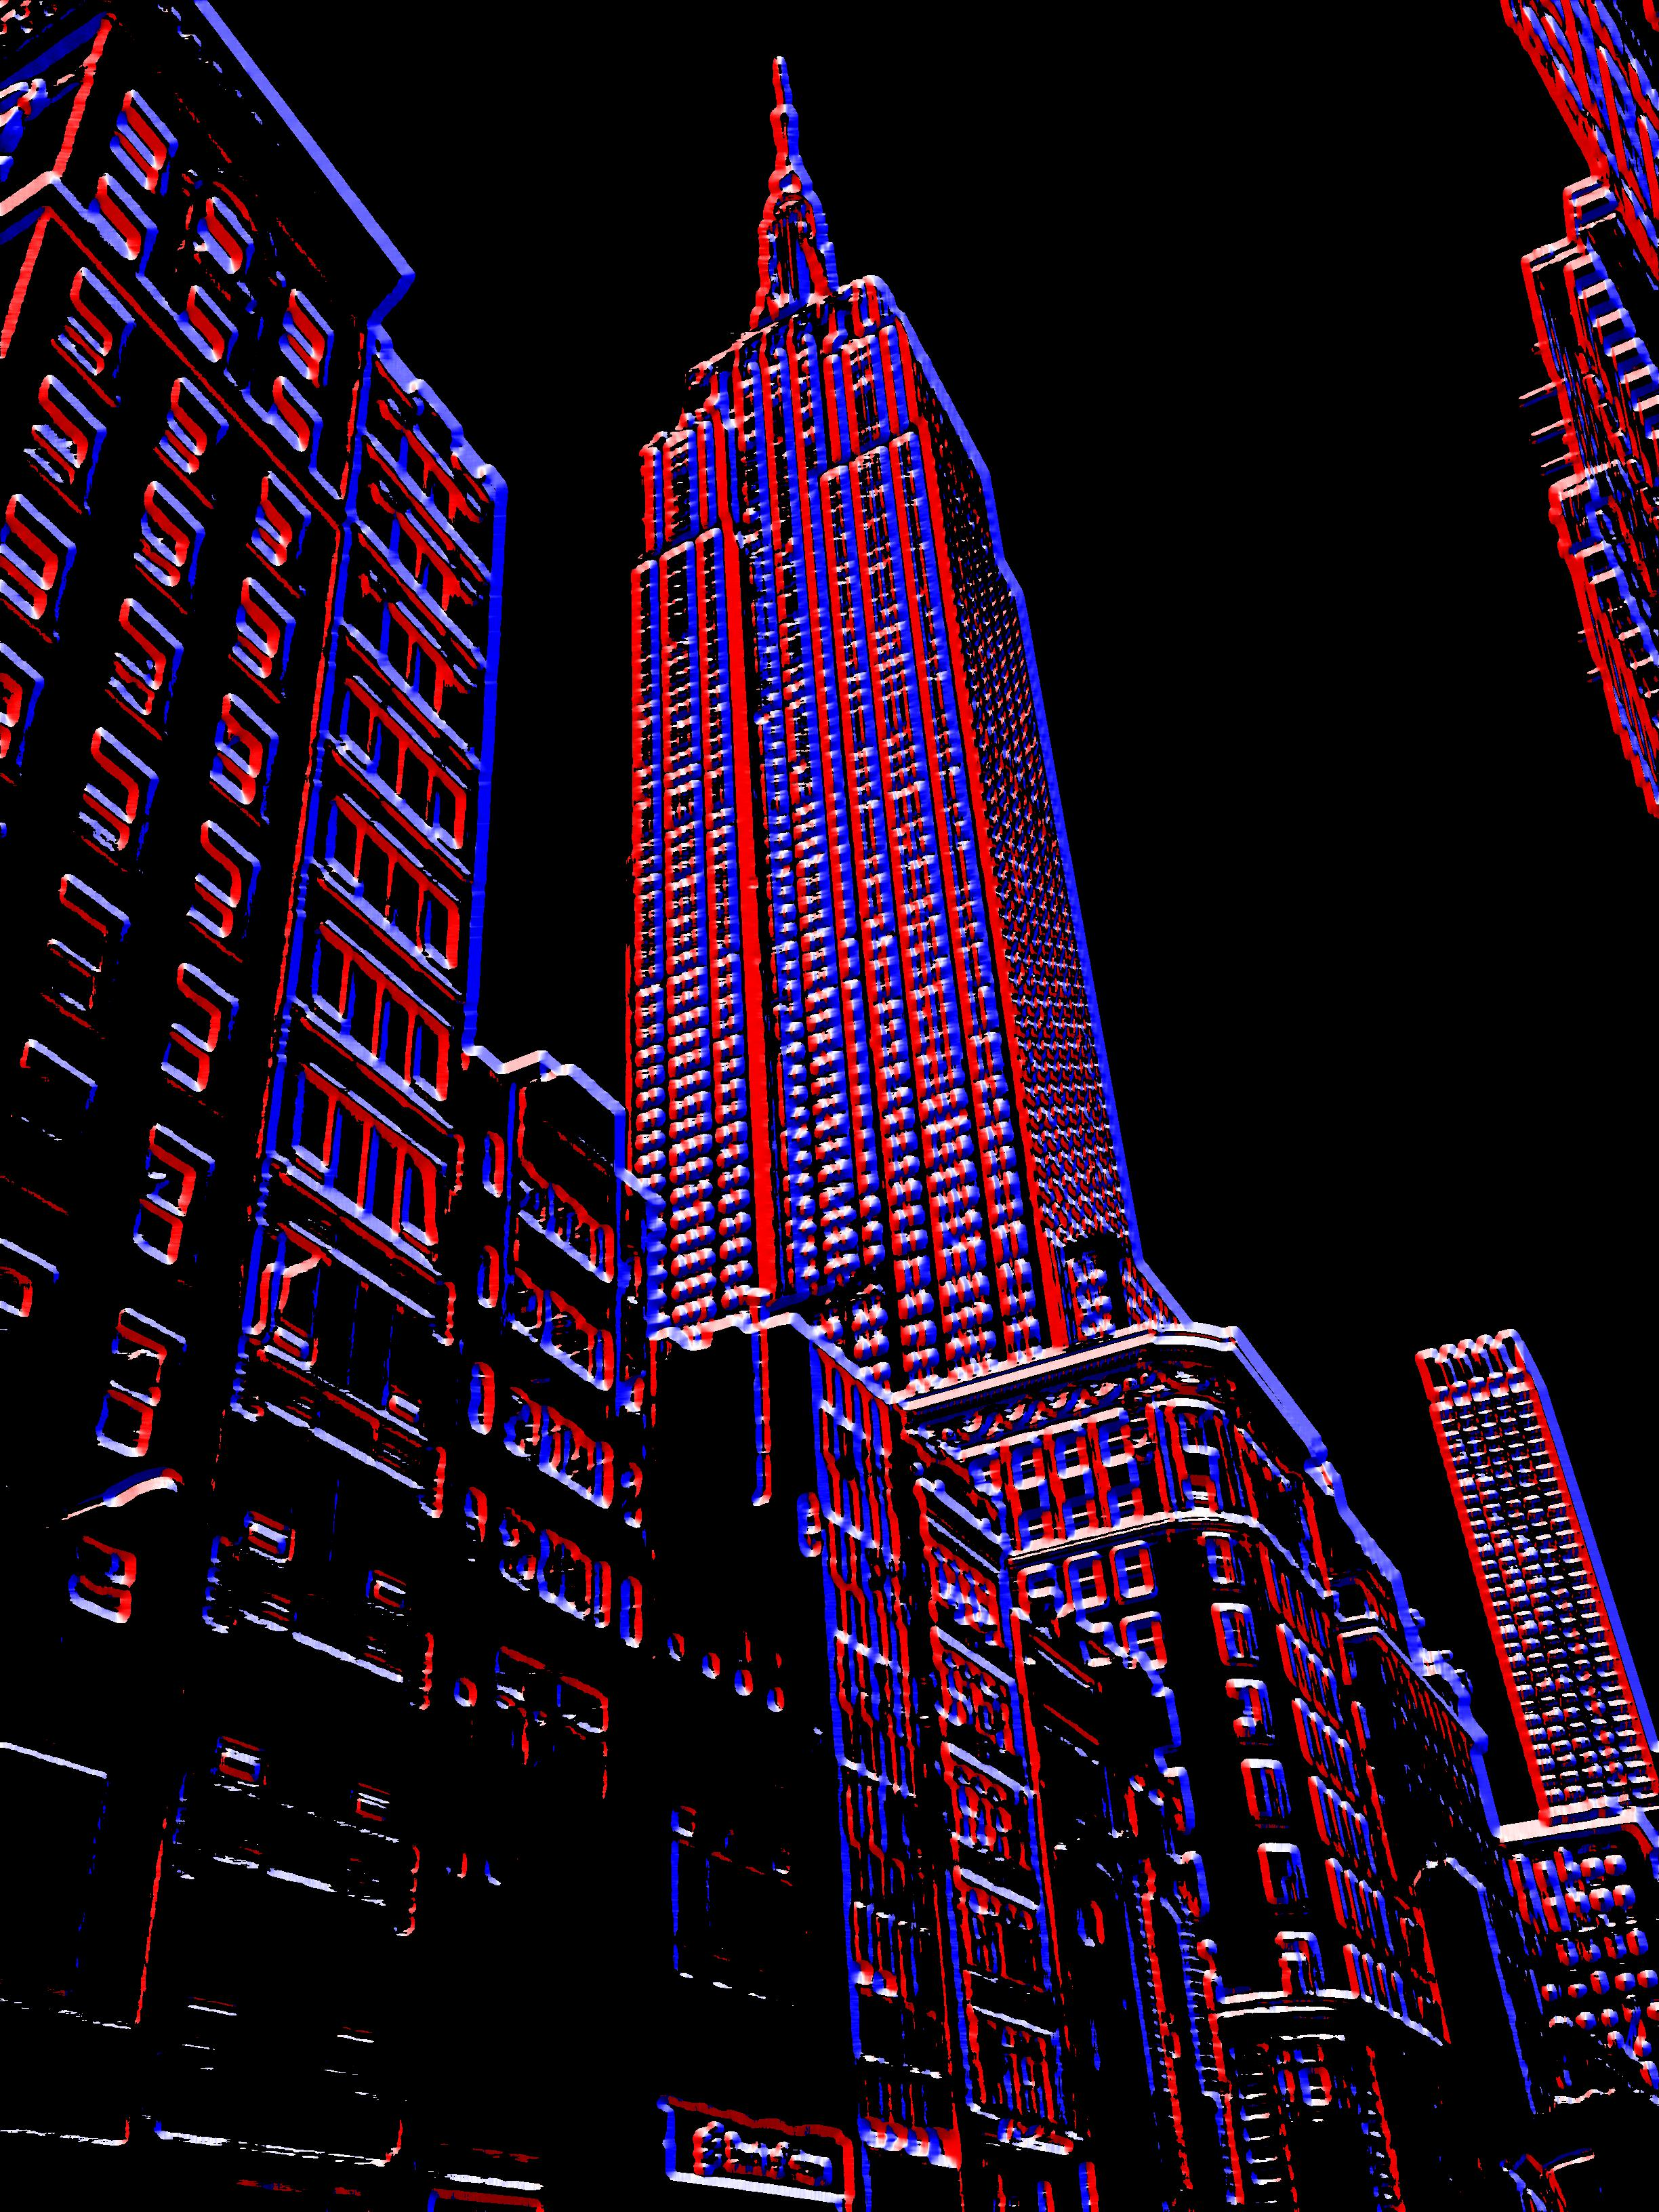
\includegraphics[height=7.3cm]{images/edge_color_1.jpg}
\caption{Coloring the edges.}
\label{fig:example}
\end{figure}

\section{Conclusion}

We have presented a systematic and artistic technique to color the edges of an image. Figure 7 displays some more examples produced by the edge coloring pipeline. This approach leverages both the gradient magnitude and direction to color edges. By enhancing image gradients with color, we can better visualize edges and create new artistic renderings of images.

\begin{figure}[h!]
\centering
\subfloat{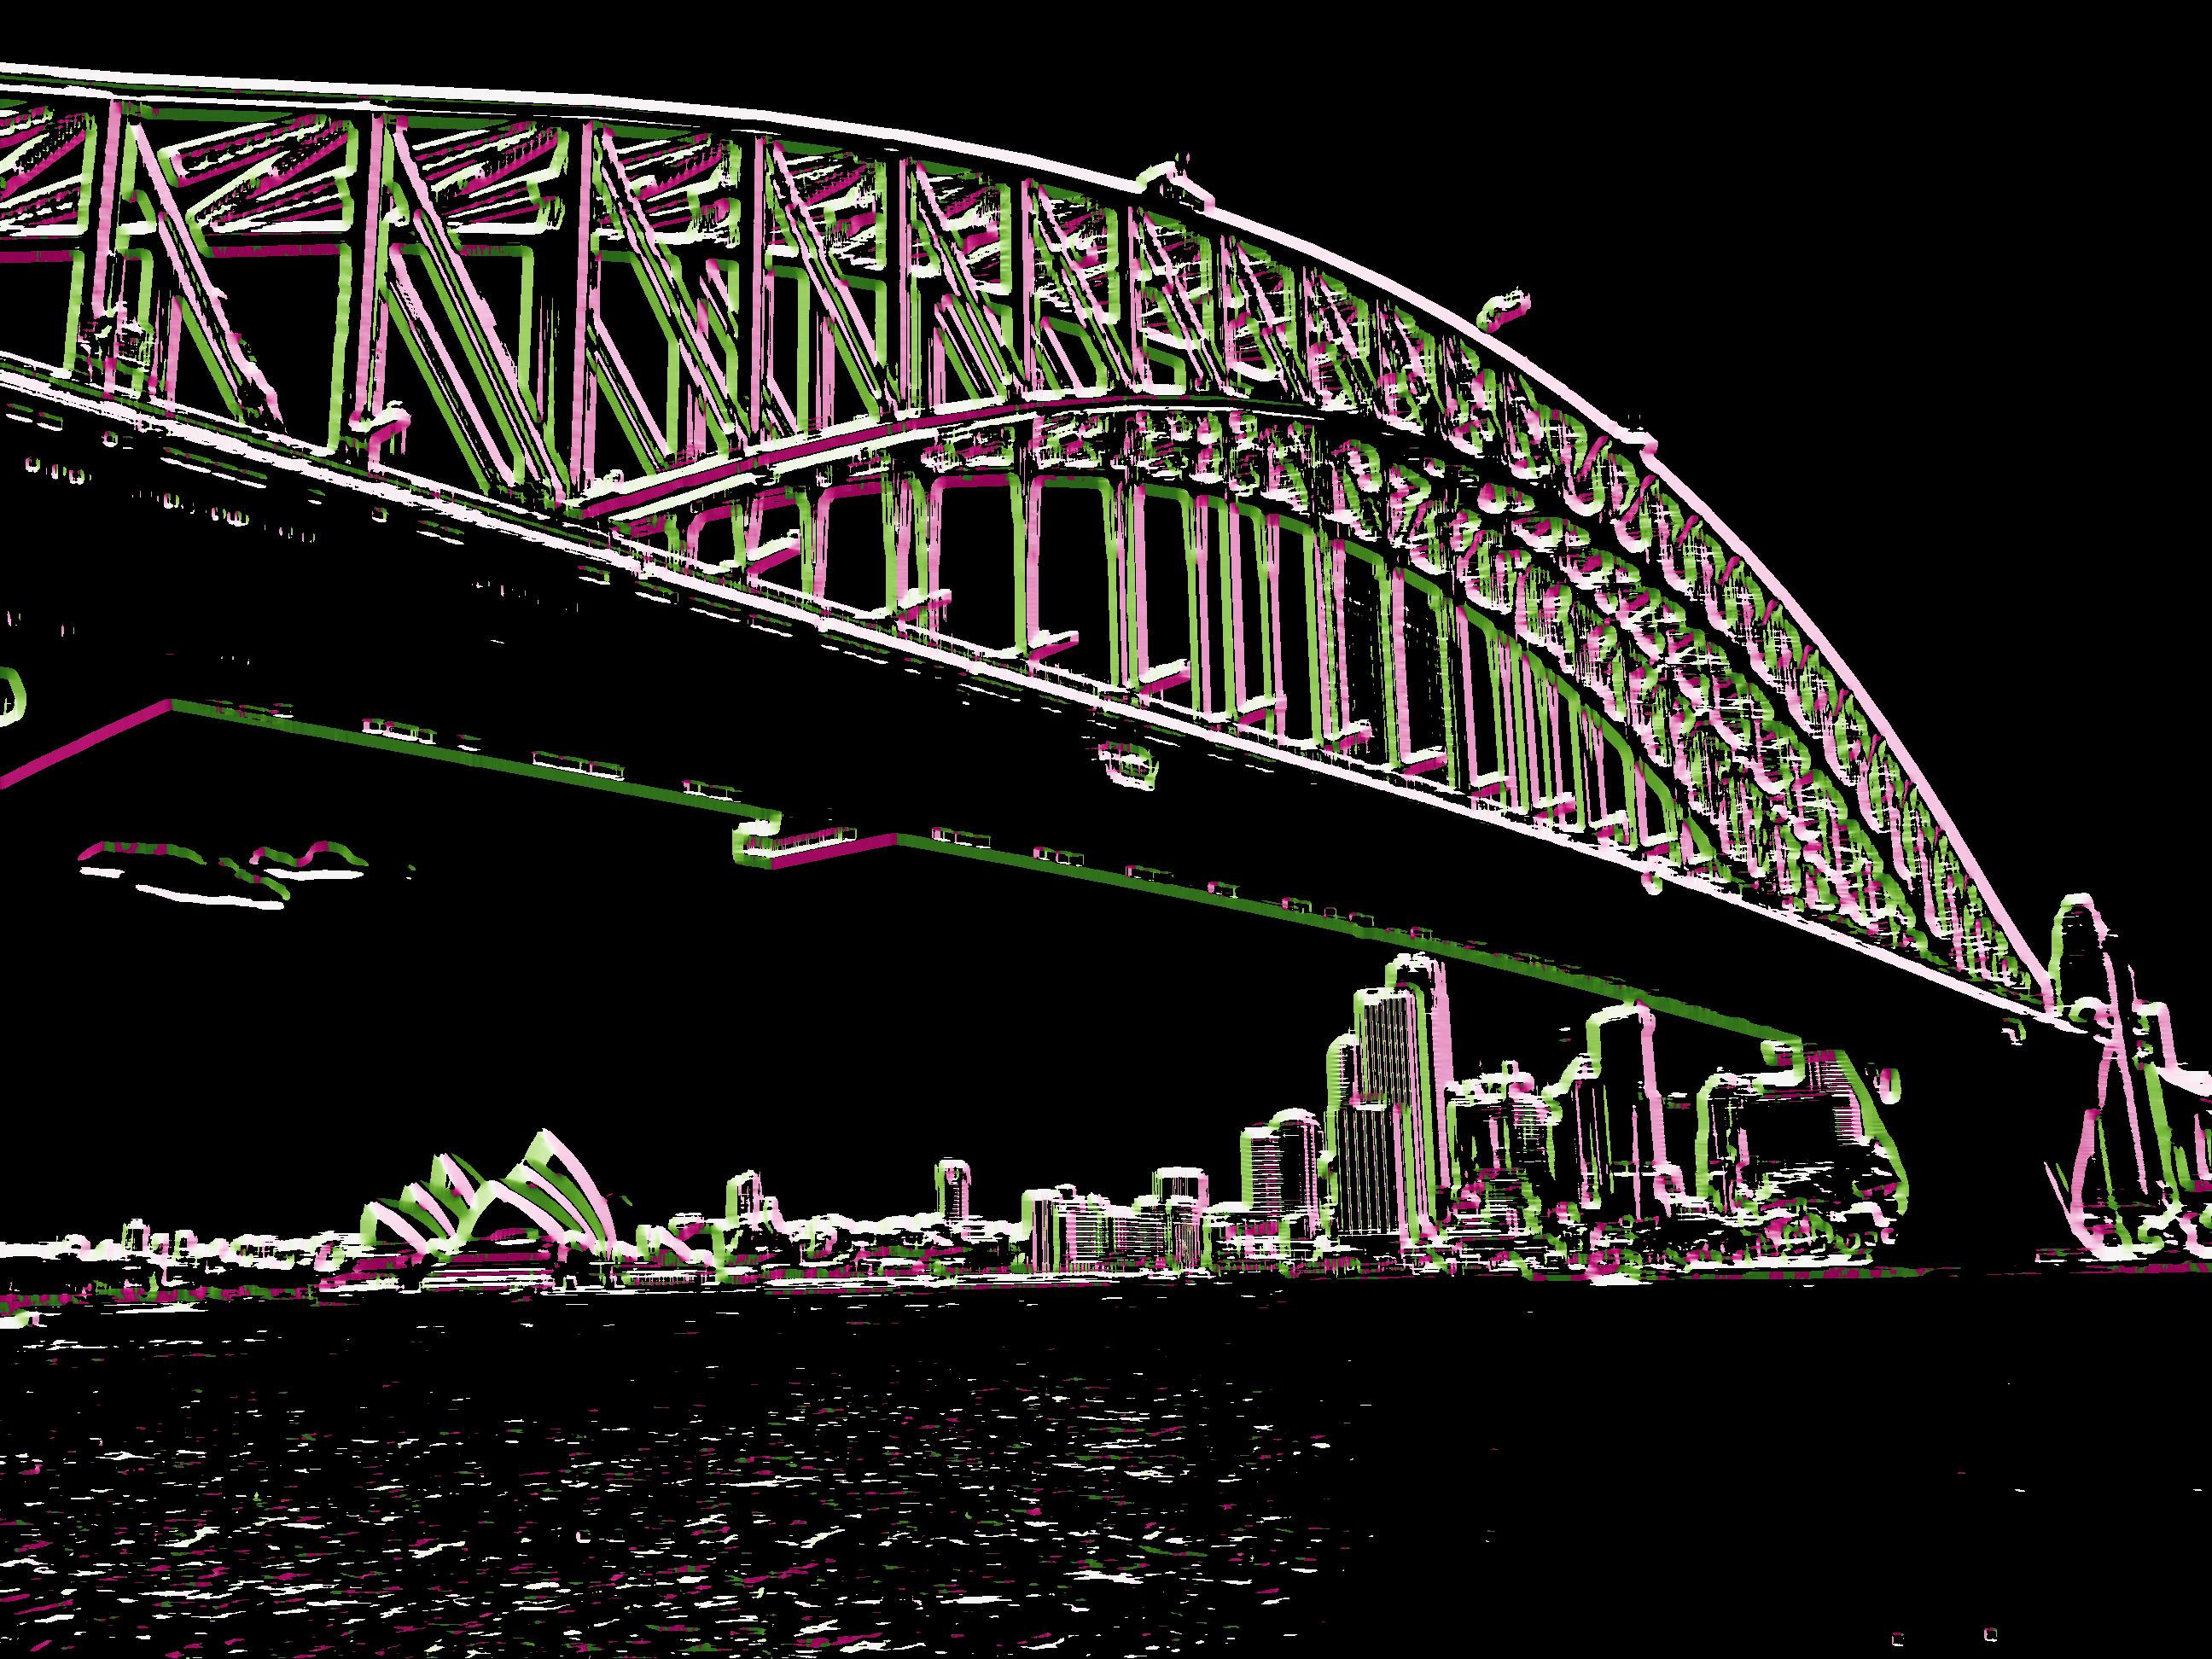
\includegraphics[height=5.2 cm]{images/edge_color_3.jpg}} \\
\subfloat{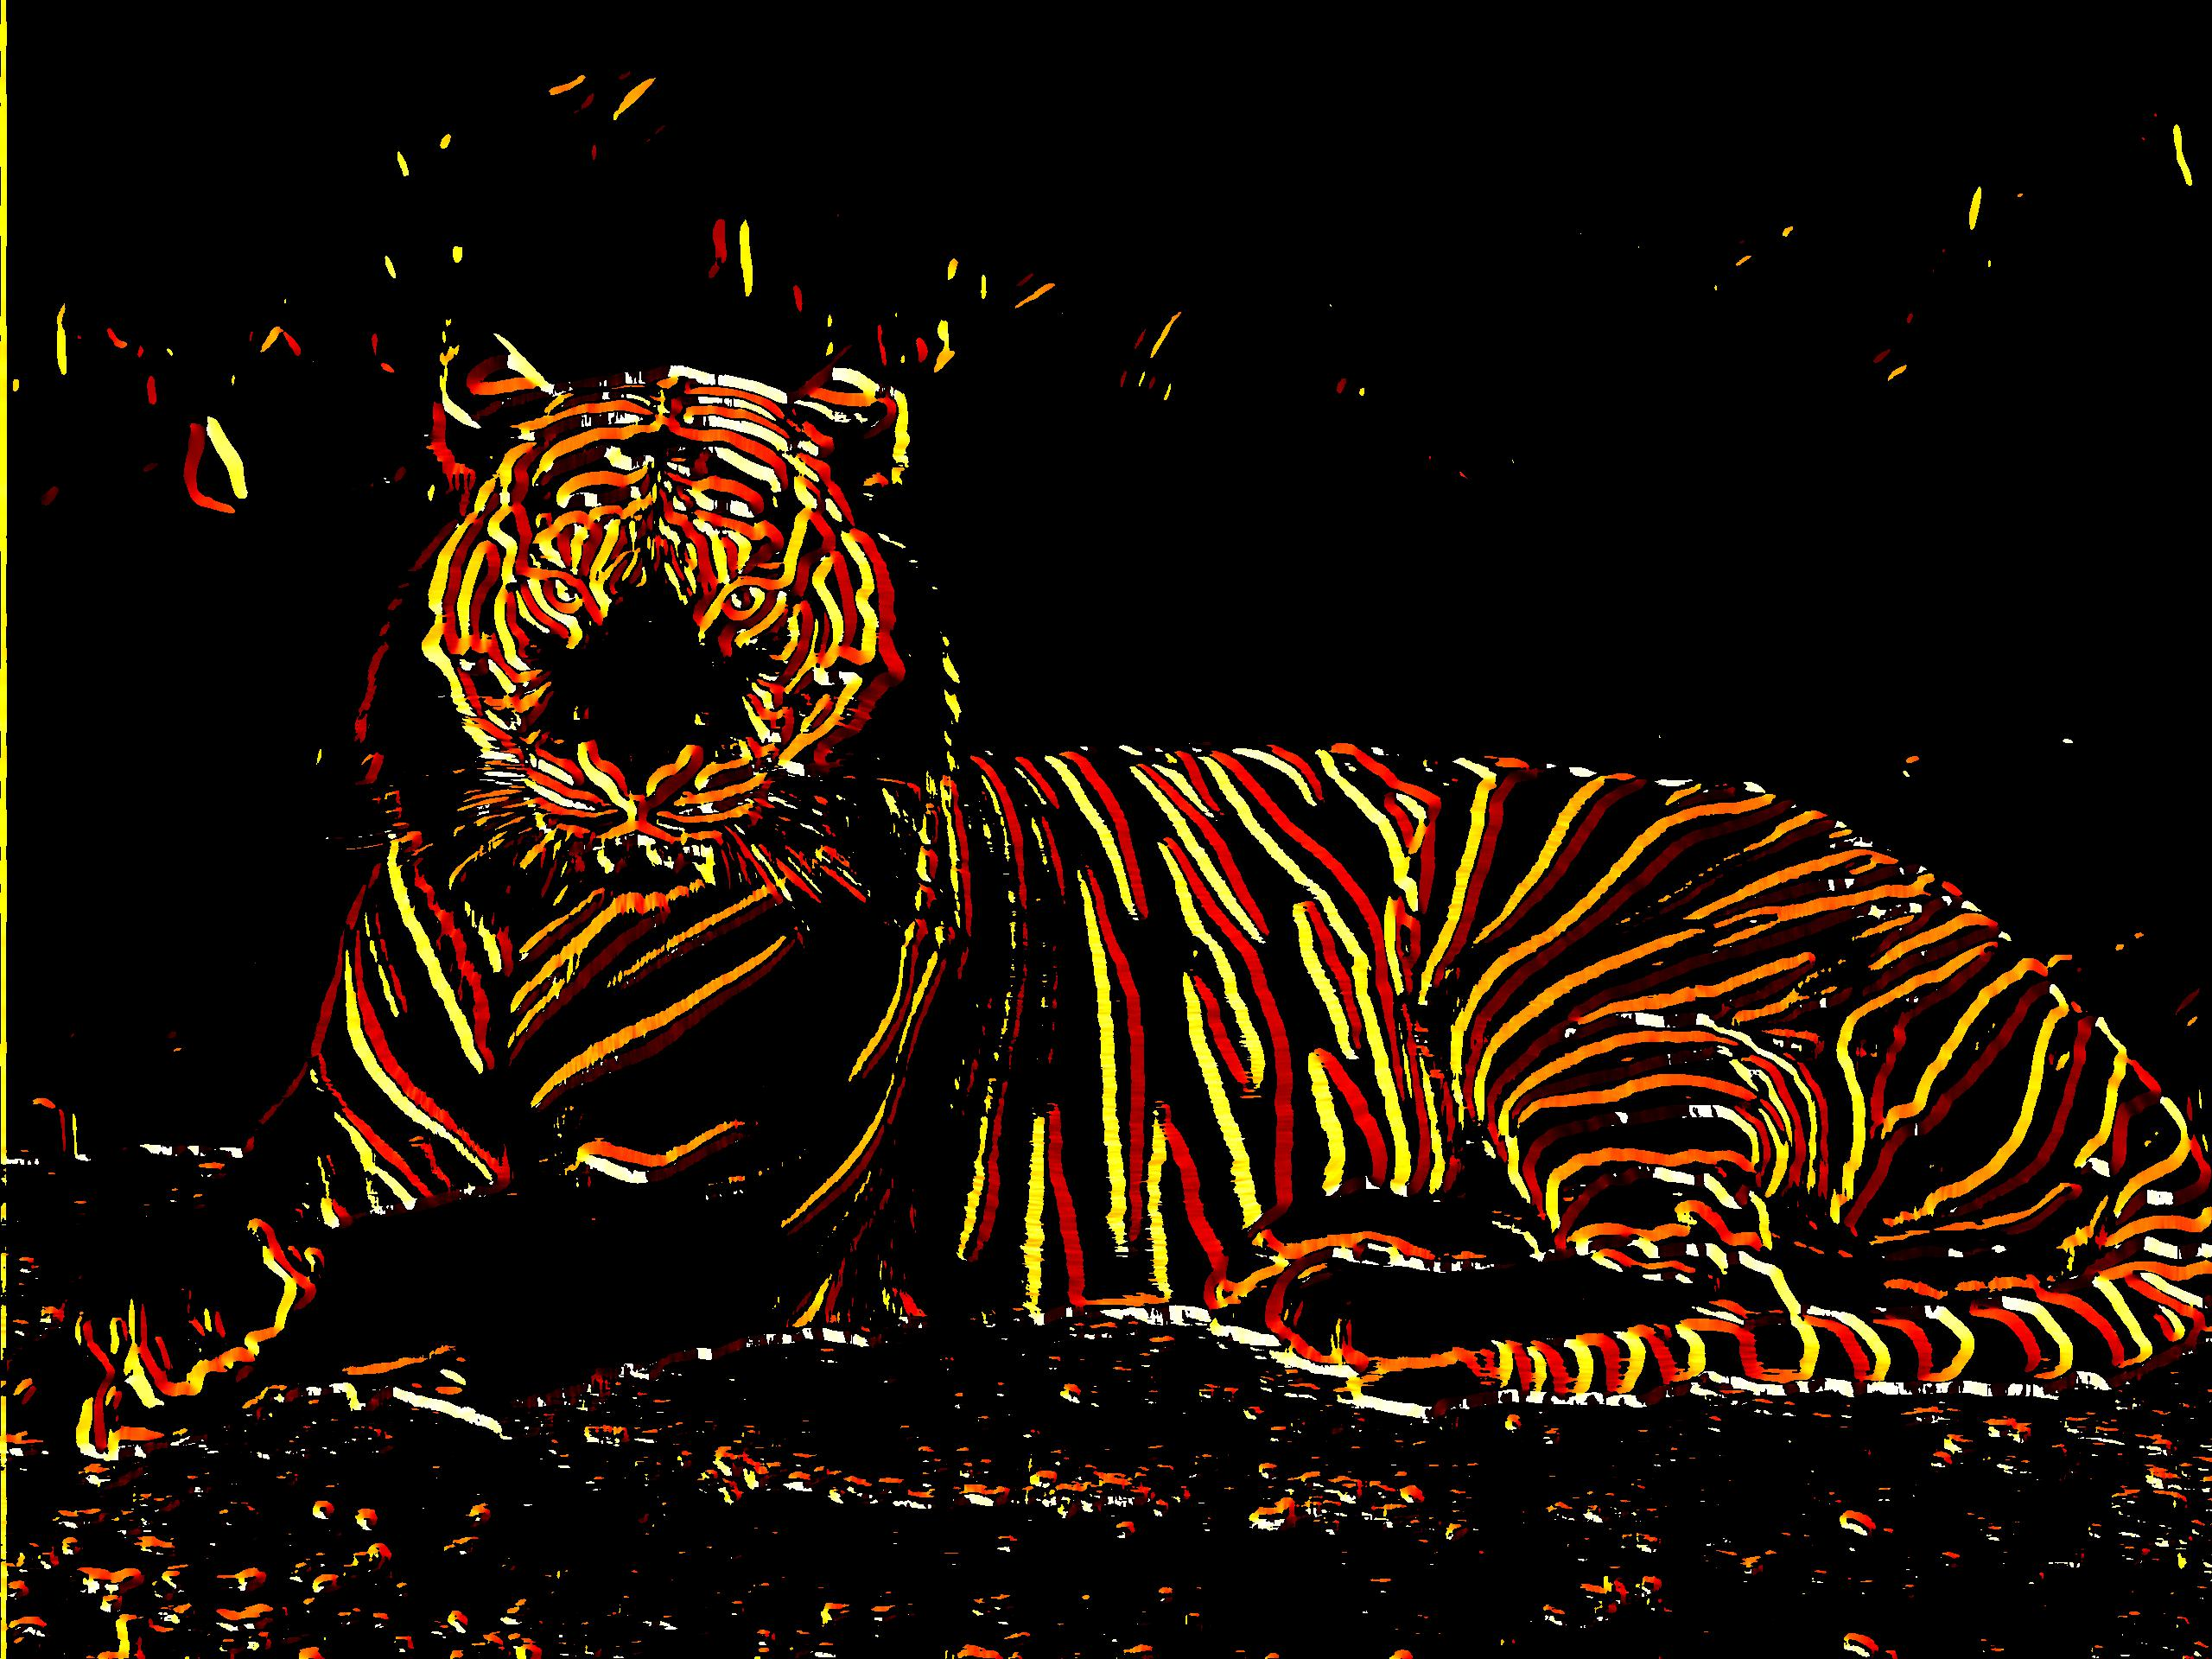
\includegraphics[height=5.2 cm]{images/edge_color_2.jpg}} \\
\subfloat{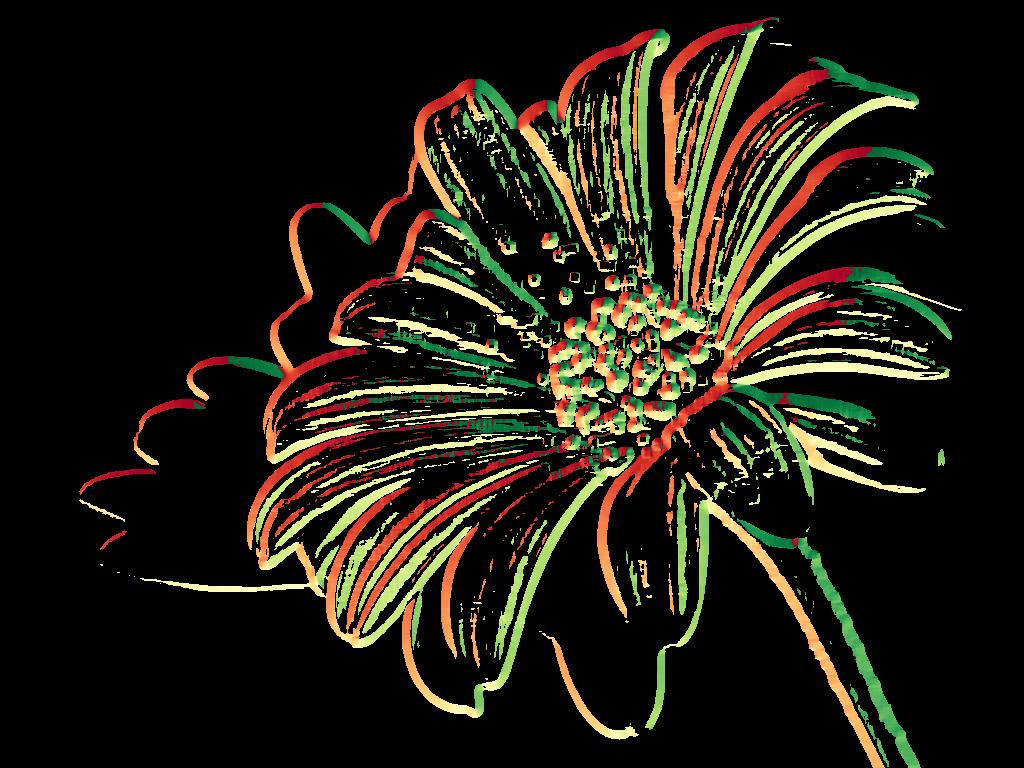
\includegraphics[height=5.2 cm]{images/edge_color_4.jpg}}
\caption{Results from edge coloring pipeline.}
\label{fig:example}
\end{figure}

\clearpage

\bibliographystyle{splncs}
\bibliography{egbib}
\end{document}
